\section{Experimental Results and Discussion}

%%%% BECHMARKS
\begin{table*}[t]
\begin{center}
\begin{small}
\begin{tabular}{llll}
\hline
\textbf{Task}  & \textbf{Benchmark} & \textbf{\textit{In-domain} Test set} & \textbf{\textit{Out-of-domain} Test set} \\ \hline
\pos (\accuracy)    & \best{0.972} \cite{Toutanova:2003} & 0.959 (\Skipgram[\withup]) & 0.910 (\Skipgram)\\ 
\chunking (\fscore) & \best{0.942} \cite{Sha:2003} & 0.938 (\brown[b = 2000]) & 0.676 (\Glove)\\  
\ner (\fscore)      & \best{0.893} \cite{Ando:2005} & 0.868 (\Skipgram) & 0.736 (\Skipgram) \\  
\mwe (\fscore)      &0.625 \cite{Schneider+:2014} & \best{0.654} (\CW) & --- \\ %
\hline
\end{tabular}
\caption{State-of-the-art results vs.\ our best results for in-domain and
  out-of-domain test sets.}
\label{benchmark}
\end{small}
\end{center}
\end{table*}


%%%%%%%%%%%%%%%%%%%%%%%%%%%%
%%% HEATMAPS 
\begin{figure*}[t!]
\centering
\begin{subfigure}{7cm}
	\centering
    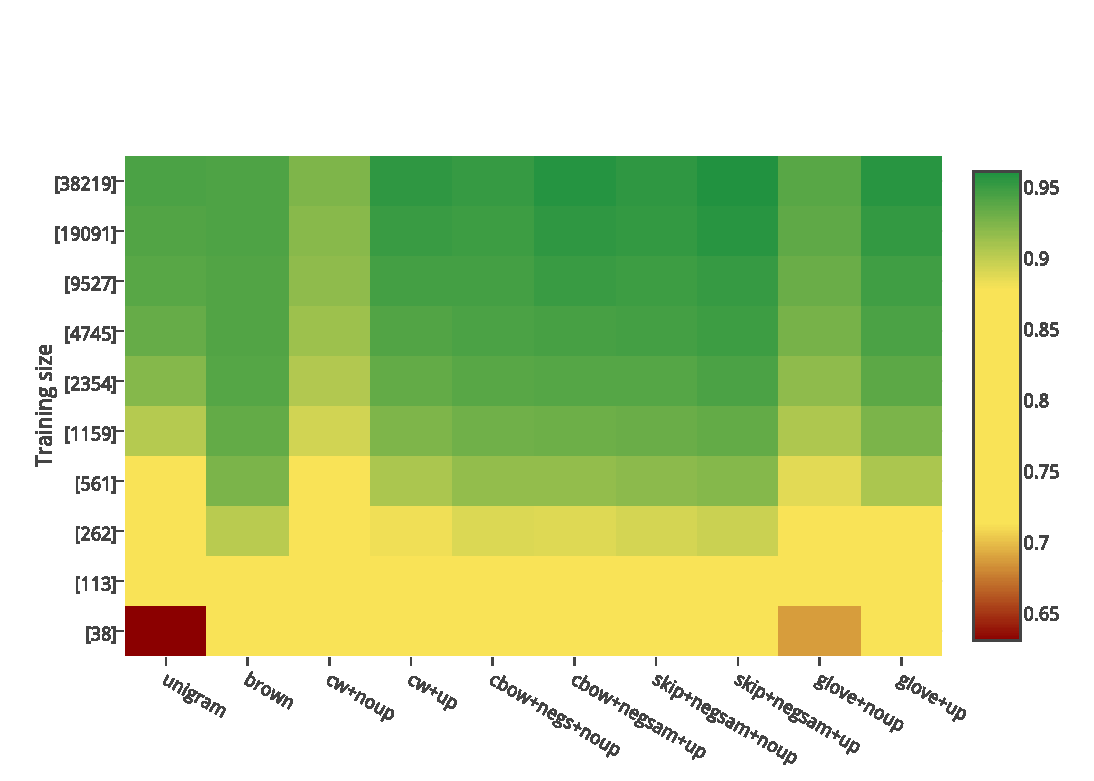
\includegraphics[scale=0.38]{plots/map-pos-color-invert}    	
	\subcaption{\pos (\accuracy)}	
	\label{pos}
\end{subfigure}
\begin{subfigure}{7cm}
	\centering
    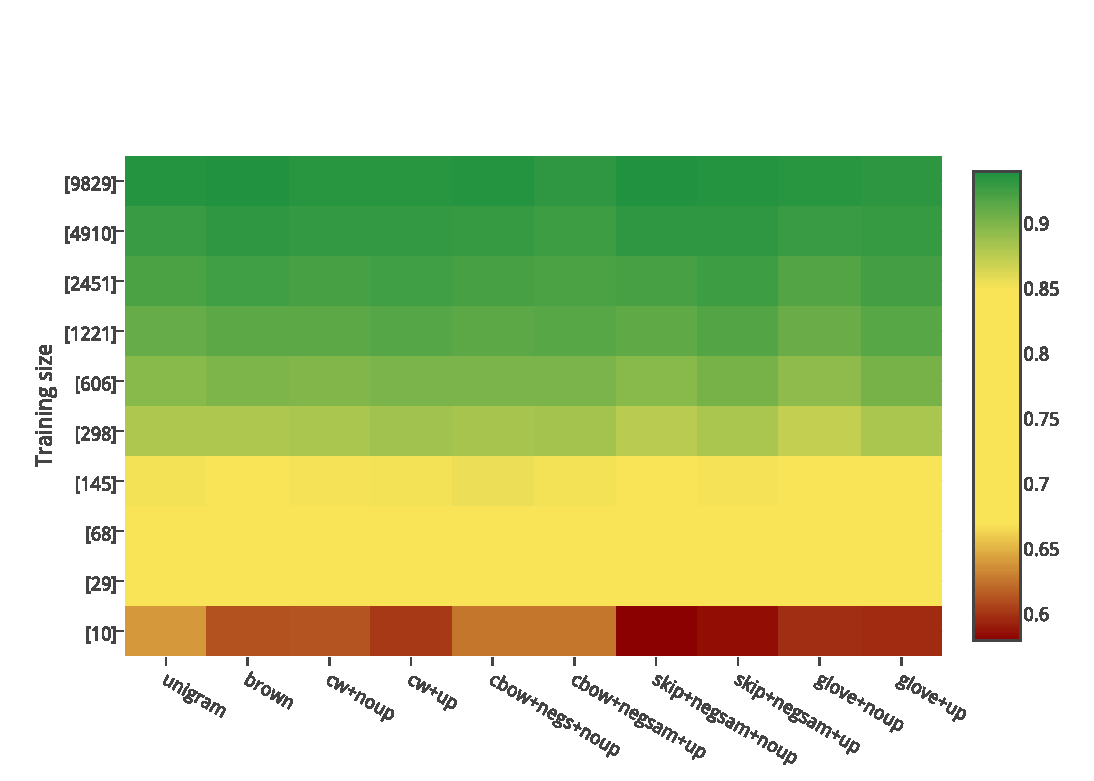
\includegraphics[scale=0.38]{plots/map-chunk-color-invert}
	\subcaption{\chunking (\fscore)}	
	\label{chu}
\end{subfigure}
%\\[-.5ex]  %%<-- in this line
\begin{subfigure}{7cm}
	\centering
    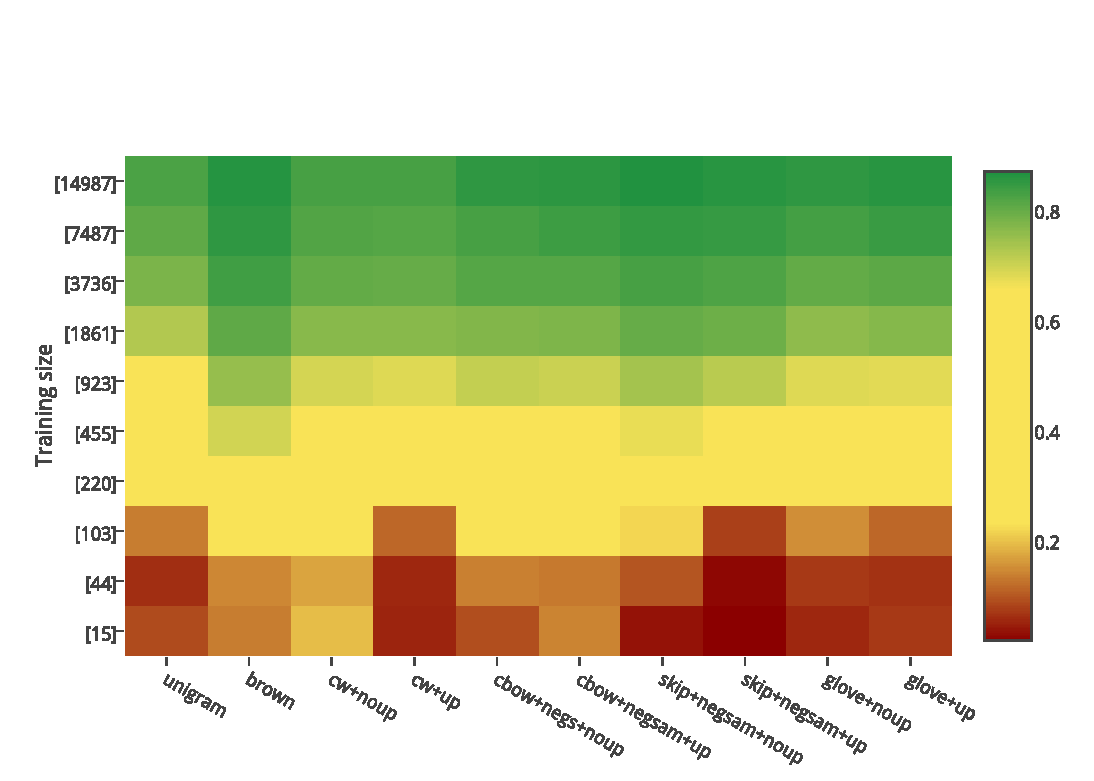
\includegraphics[scale=0.38]{plots/map-ner-color-invert}    	
	\subcaption{\ner (\fscore)}	
	\label{ner}
\end{subfigure}
\begin{subfigure}{7cm}
	\centering
    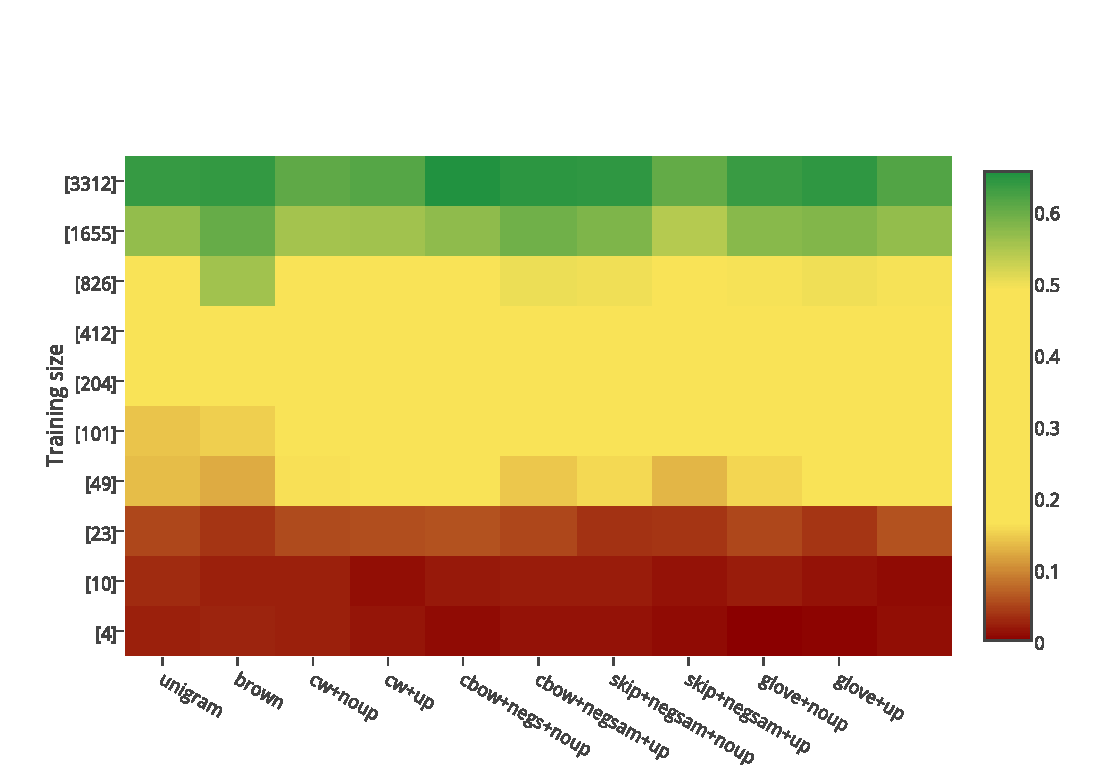
\includegraphics[scale=0.38]{plots/map-mwe-color-invert}
	\subcaption{\mwe (\fscore)}		
	\label{mwe}
\end{subfigure}
\caption{Results for each type of word representation over \pos, \chunking, \ner and
  \mwe, optionally with updating (``\withup''). The $y$-axis indicates the training data
  sizes (on a log scale). Green = high performance, and red = low
  performance, based on a linear scale of the best- to worst-result for
  each task. }
\label{fig:heatmaps}
\end{figure*}

%%%%%%%%%%%%%%%%%%%%%%%%%%%%
%%% OOV 
\begin{figure*}[t!]
\centering
    	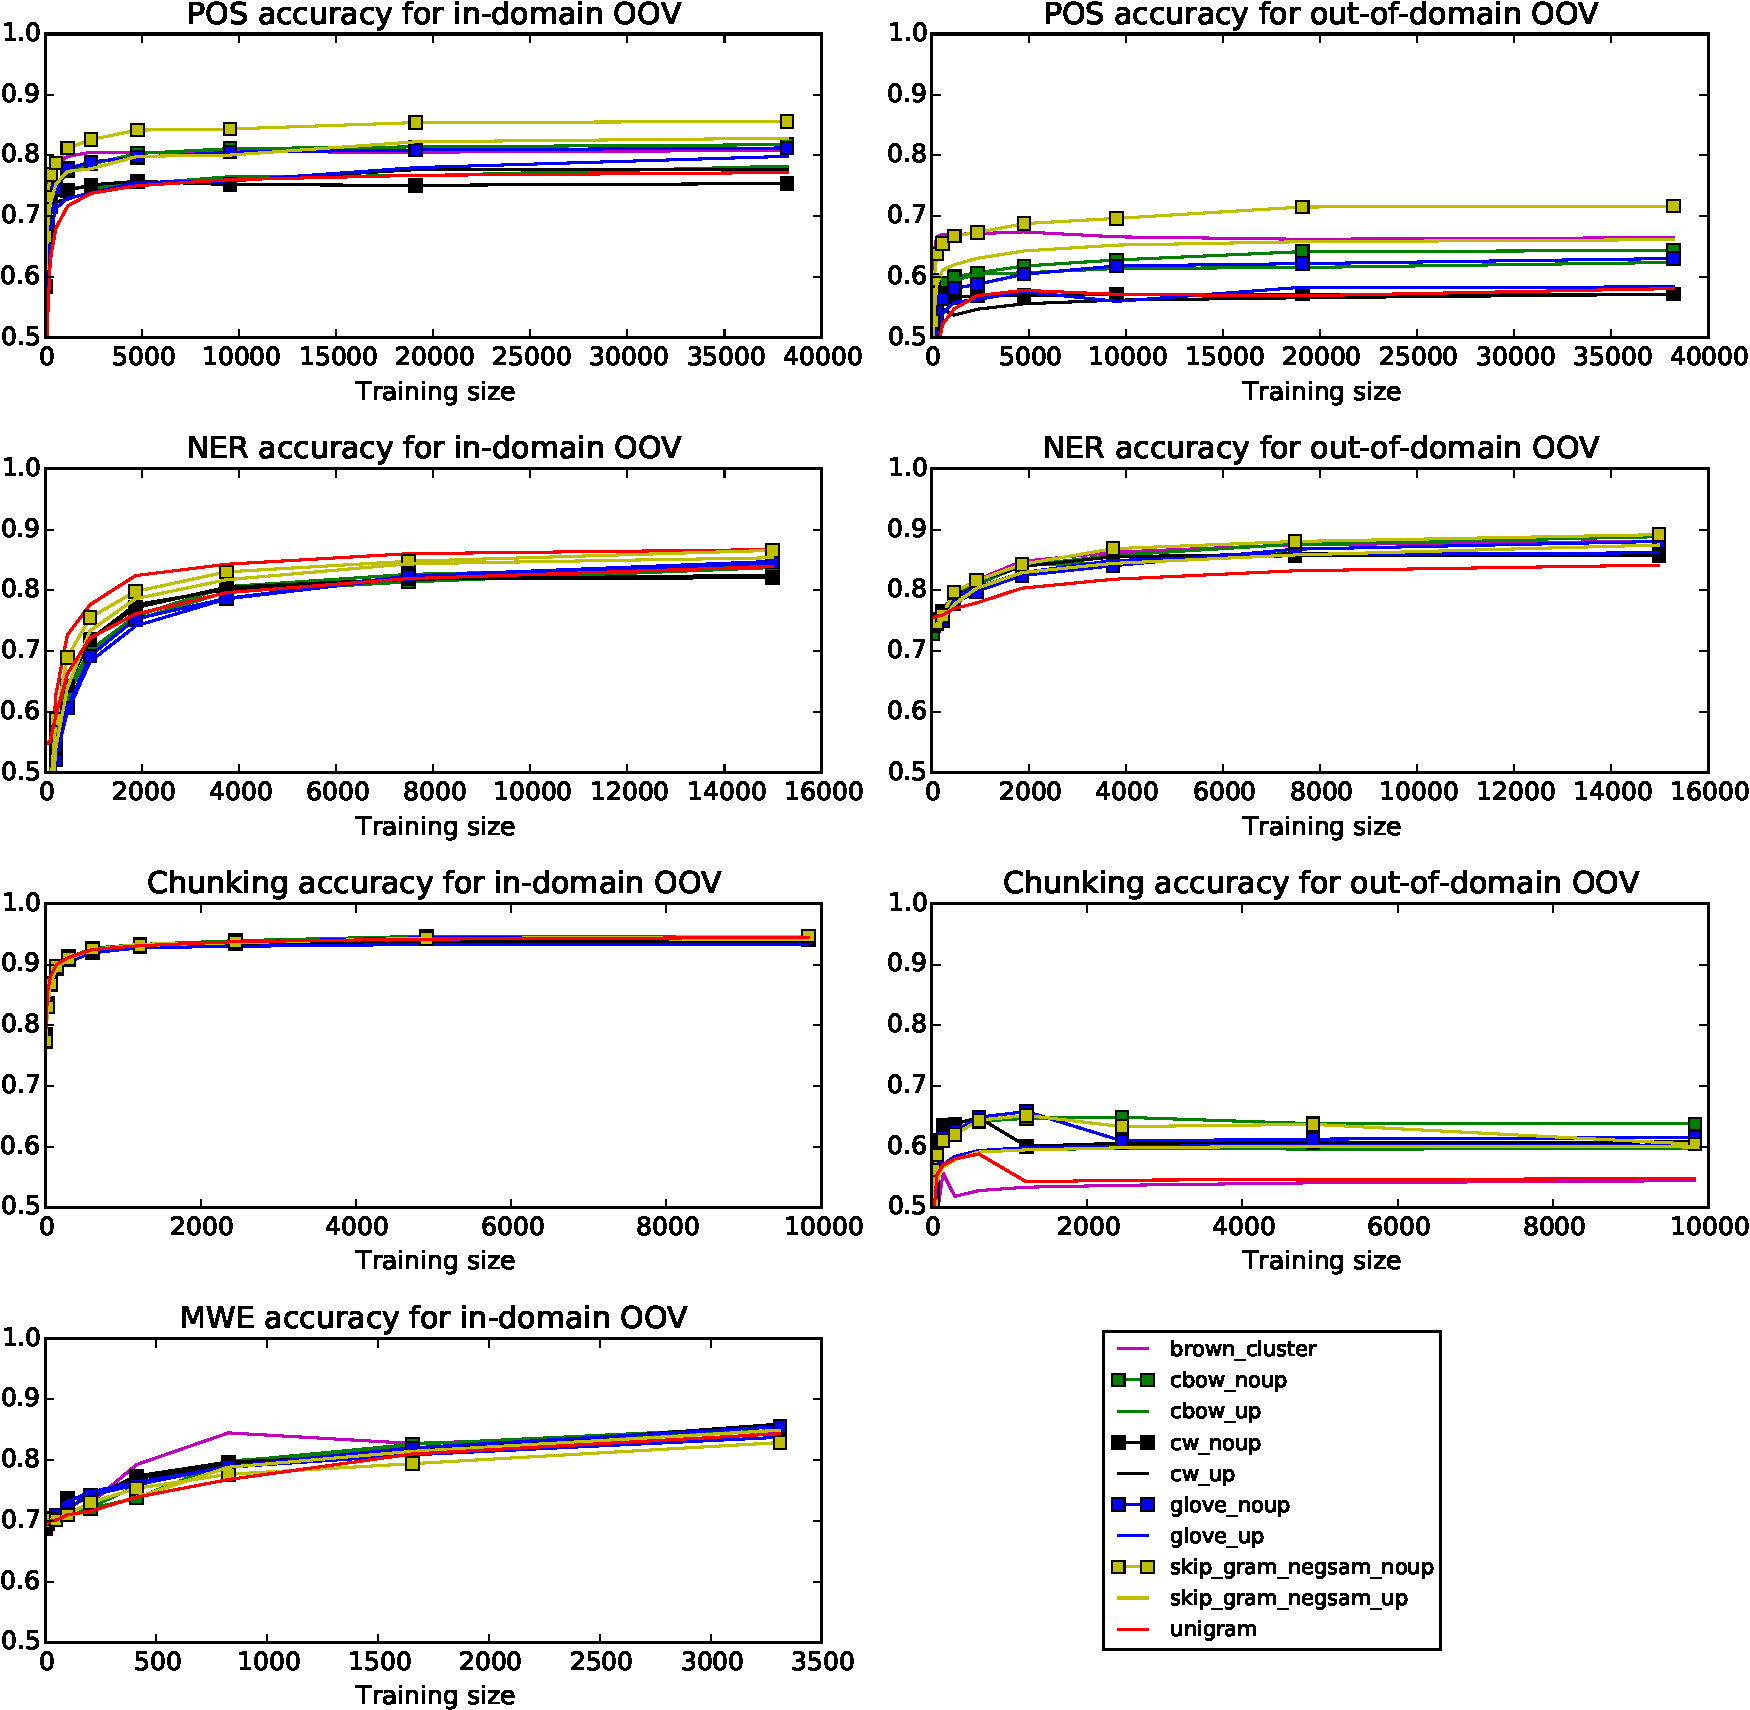
\includegraphics[scale=0.5]{plots/OOV-plots}
\caption{\accuracy over out-of-vocabulary (OOV) words for \textit{in-domain} and \textit{out-of-domain} test sets.}
\label{OOV} 
\end{figure*}



We structure our evaluation by stepping through each of our five
research questions (\RQ[1--5]) from the start of the paper. In this, we
make reference to: (1) the best-performing method both in- and
out-of-domain vs.\ the state-of-the-art (\tabref{benchmark}); (2) a
heat map for each task indicating the convergence rate for each word
representation, with and without updating (\figref{fig:heatmaps}); 
(3) OOV accuracy both in-domain and out-of-domain for each task
(\figref{OOV}); and (4)  visualisation of the impact of
updating on word embeddings, based on t-SNE
(\figref{fig:vectorfield}).

%\textbf{(i) Are the evaluated word embedding methods better than unigram features?}
\paragraph{\RQ[1]: Are word embeddings better than one-hot unigram features
  and Brown clusters?}  As shown in \tabref{benchmark}, the
best-performing method for every task except in-domain \chunking is a
word embedding method, although the precise method varies
greatly. \figref{fig:heatmaps}, on the other hand, tells a more subtle
story: the difference between \unigram and the other word
representations is relatively modest, esp.\ as the amount of training
data increases. Additionally, the difference between \brown and the word
embedding methods is modest across all tasks. So, the overall answer
would appear to be: yes for unigrams when there is little training data, but not really for \brown.




%\textbf{(ii) How does the size of labelled training data affect the experimental results?}
\paragraph{\RQ[2]: Do word embedding features require less training data?}
\figref{fig:heatmaps} shows that for \pos and \ner, with only several hundred training instances, 
word embedding features achieve superior results to \unigram. 
For example, when trained with 561 instances, the \pos model using \Skipgram[\withup] embeddings is 5.3\% above
\unigram; and when trained with 932 instances, the \ner model using \Skipgram is 11.7\% above \unigram. 
Similar improvements are also found for other types of word embeddings and \brown, when the training set is small. 
However, all word representations perform similarly for \chunking
regardless of training data size.
For \mwe, \brown performs slightly better than the other methods when
trained with approximately 25\% of the training instances. 
Therefore, we conjecture that the \pos and \ner tasks benefit more from
distributional similarity than \chunking and \mwe.

\paragraph{\RQ[3]: Does task-specific updating improve all word embeddings across all tasks?}
Based on \figref{fig:heatmaps}, updating of word representations can
equally correct poorly-learned word representations, and harm
pre-trained representations, due to overfitting.
For example, \CW and \Glove perform significantly worse than \Skipgram
in both \pos and \ner without updating, but \emph{with} updating, the
gap between their results and the best performing method becomes
smaller. In contrast, \Skipgram performs worse over the test data with
updating, despite the results on the development set improving by 1\%.

To further investigate the effects of updating, we sampled 60 words and
plotted the changes in their word embeddings under updating, using 2-d
vector fields generated by using matplotlib and t-SNE \cite{vanderMaaten:Hinton:2008}. Half
of the words were chosen manually to include known word clusters such as
days of the week and names of countries; the other half were selected
randomly. Additional plots with 100 randomly-sampled words and the
top-100 most frequent words, for all the methods and all the tasks, can
be found in the supplementary material and at
\url{https://123abc123abd.wordpress.com/}.  In each plot, a single arrow
signifies one word, pointing from the position of the original word embedding to the updated representation.

In \figref{fig:vectorfield}, we show vector fields plots for \chunking and \ner using \Skipgram embeddings.
For \chunking, most of the vectors were changed with similar magnitude,
but in very different directions, including within the clusters of days of
the week and country names.
In contrast, for \ner, there was more homogeneous change in word vectors
belonging to the same cluster.
This greater consistency is further evidence that semantic homogeneity
appears to be more beneficial for \ner than \chunking. 


%%%%%%%%%%%%%%%%%%%%%%%%%%%%
%%% Vector fields
% POS
\begin{figure*}[t!]
\centering
\begin{subfigure}[b]{0.48\textwidth}
	\centering
    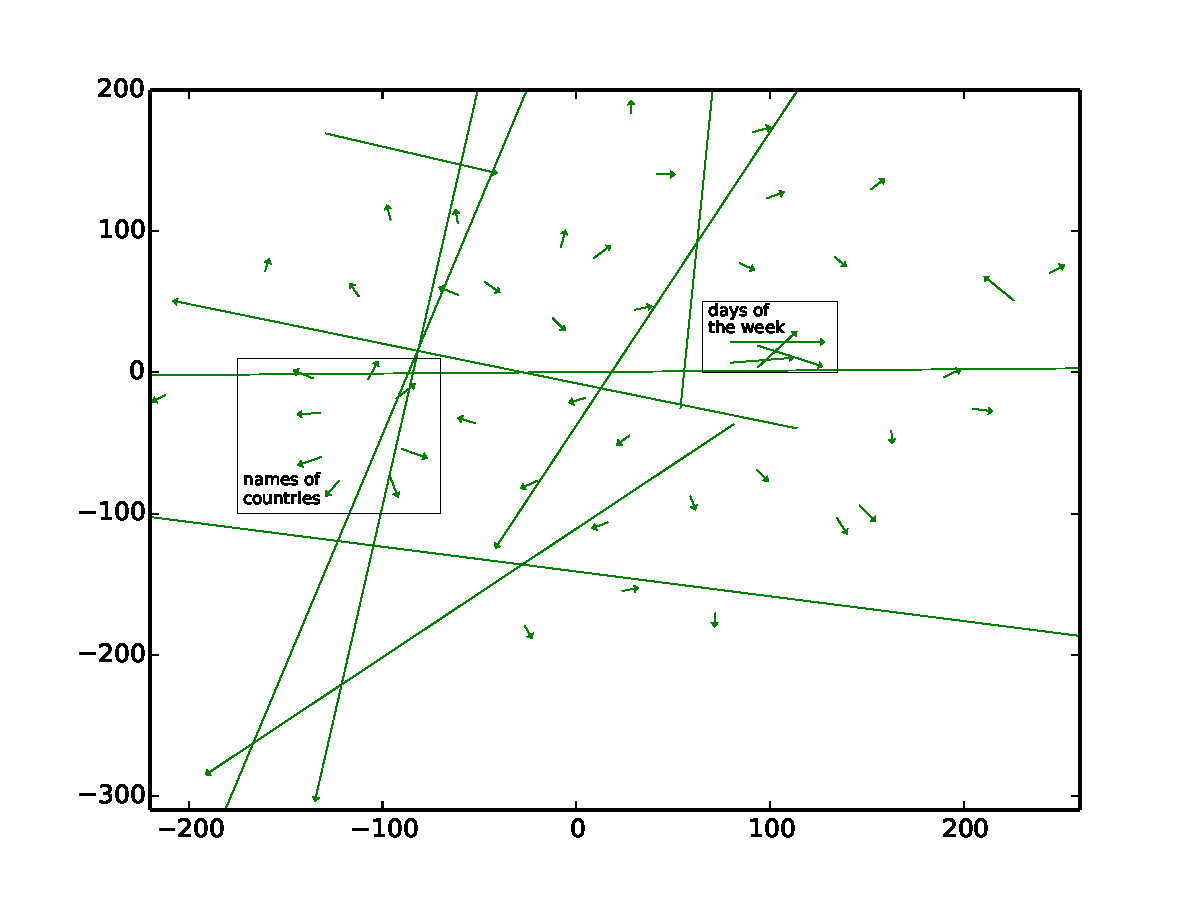
\includegraphics[width=\textwidth]{plots/vectorField/Lizhen/scaled/Lizhen_skip_chunking}
	\subcaption{\chunking}	
	\label{fig:skipChu}
\end{subfigure}
\begin{subfigure}[b]{0.48\textwidth}
	\centering
    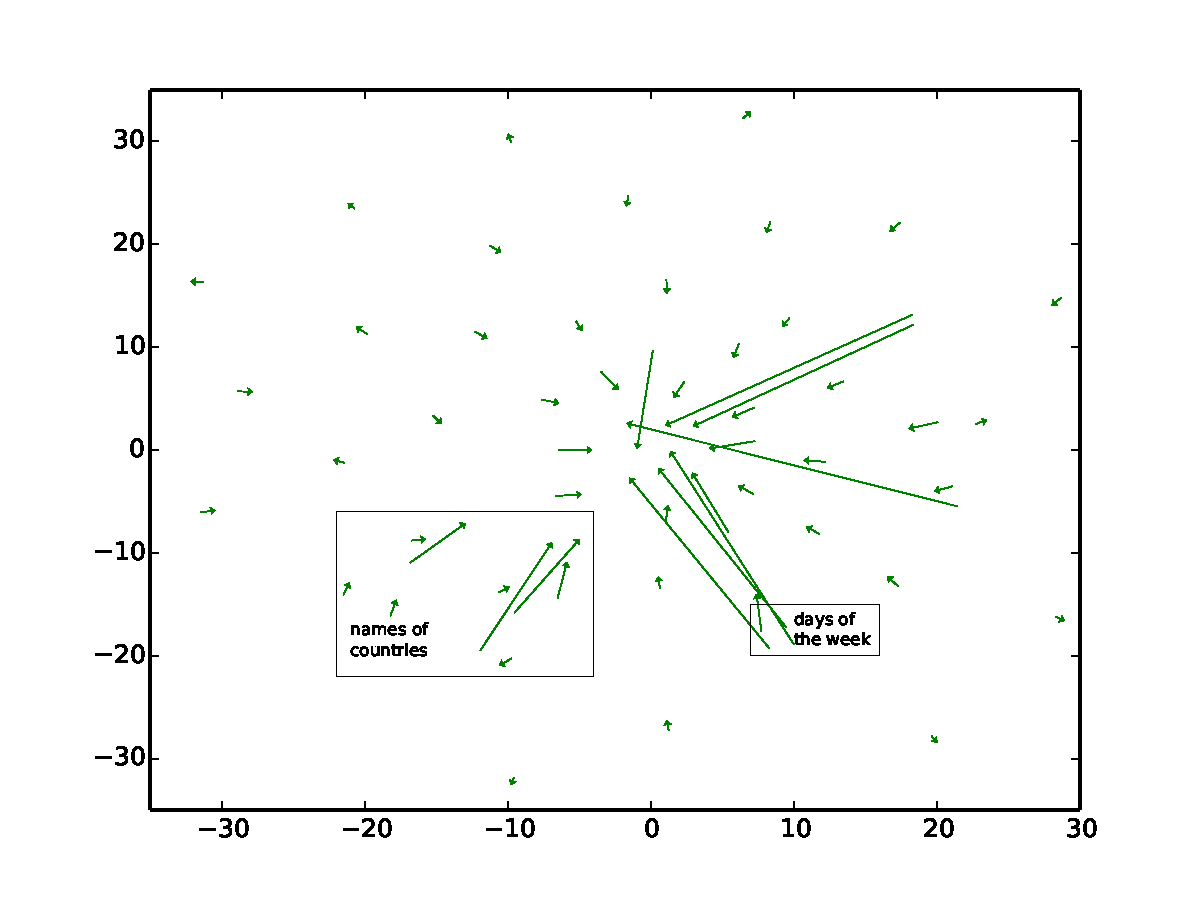
\includegraphics[width=\textwidth]{plots/vectorField/Lizhen/Lizhen_skip_NER}    	
	\subcaption{\ner}
	\label{fig:skippos}	
\end{subfigure}
%\begin{subfigure}[b]{0.48\textwidth}
%	\centering
%   \includegraphics[width=\textwidth]{plots/vectorField/skip_\ner.png}
%	\label{fig:skipner}
%	\subcaption{}	
%\end{subfigure}
%%\begin{subfigure}{6cm}
%	\centering
 %   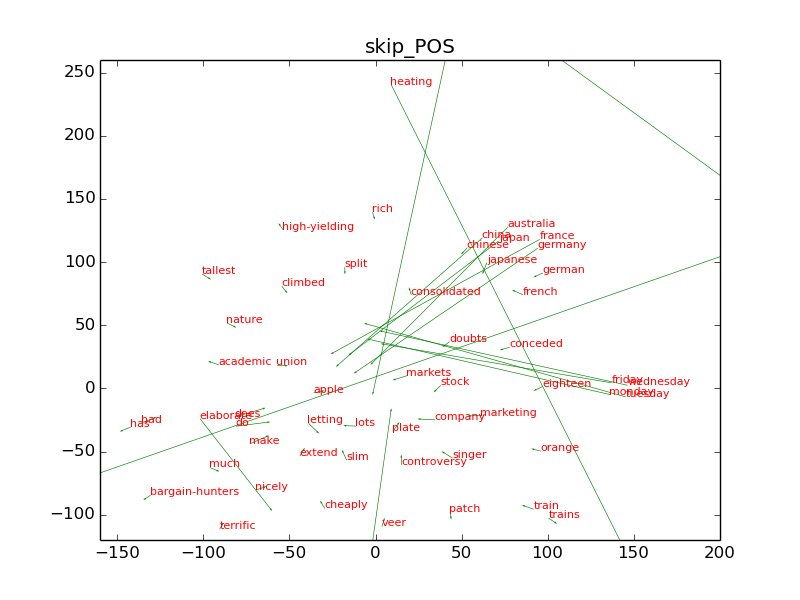
\includegraphics[scale=0.3]{plots/vectorField/skip_POS.png}
%	\label{fig:skipmwe}
%	\subcaption{}	
%\end{subfigure}
\caption{A t-SNE plot of the impact of updating on \Skipgram}
\label{fig:vectorfield}
\end{figure*}


% This also indicates that the graph transformer can identify useful factors in word representations and keep them during training.
\paragraph{\RQ[4]: What is the impact of word embeddings cross-domain
  and for OOV words?}
As shown in \tabref{benchmark}, results predictably drop when we
evaluate out of domain.
The difference is most pronounced for \chunking, where there is an
absolute drop in \fscore of around 30\% for all methods, indicating that
word embeddings and unigram features provide similar information for
\chunking. 

Another interesting observation is that updating often hurts
out-of-domain performance because the distribution between domains is different. 
This suggests that, if the objective is to optimise performance across
domains, it is best not to perform updating. 

We also analyze performance on OOV words both in-domain and
out-of-domain in \figref{OOV}.
As expected, word embeddings and \brown excel in out-of-domain OOV performance.
Consistent with our overall observations about cross-domain
generalisation, the OOV results are better when updating is not performed. 

%\textbf{(ii) How does the size of labelled training data affect the experimental results?}
\paragraph{\RQ[5] Overall, are some word embeddings better than others?}
Comparing the different word embedding techniques over our four sequence
labelling tasks, for the different evaluations (overall, out-of-domain
and OOV), there is no clear winner among the word embeddings -- for
\pos, \Skipgram appears to have a slight advantage, but this does not
generalise to other tasks.\\

While the aim of this paper was not to achieve the state of the art over
the respective tasks, it is important to concede that our best
(in-domain) results for \ner, \pos and \chunking are
slightly worse than the state of the art
(\tabref{benchmark}). The 2.7\% difference between our \ner system and
the best performing system is due to the fact that we use a first-order
instead of a second-order CRF~\cite{Ando:2005}, and for the other tasks,
there are similarly differences in the learner and the complexity of the
features used.
Another difference is that we tuned the hyperparameters with random
search, to enable replication using the same random seed.
In contrast, the hyperparameters for the state-of-the-art methods are
tuned more extensively by experts, making them more difficult to reproduce.









%%% Local Variables: 
%%% mode: latex
%%% TeX-PDF-mode: t 
%%% TeX-master: "WordEmbEvaluation"
%%% End: 
